%%%%%%%%%%%%%%%%%%%%%%%%%%%%%%%%%%%%%%%%%%%%%%%%
% COPYRIGHT: (C) 2020 FAU FabLab
% CC-BY-SA 3.0
%%%%%%%%%%%%%%%%%%%%%%%%%%%%%%%%%%%%%%%%%%%%%%%%


\newcommand{\basedir}{fablab-document}
\documentclass{\basedir/fablab-document}

\renewcommand{\texteuro}{\euro}

\renewcommand{\todo}[1]{\textbf{\color{red}{TODO: #1}}}
\newcommand{\pfeil}{\ensuremath{\rightarrow}}

\date{2020}
\author{}
\fancyfoot[L]{kontakt@fablab.fau.de}
\title{Einweisung Nähmaschine Pfaff 260}


\begin{document}
\maketitle



{\LARGE  \todo{ACHTUNG UNFERTIG - Es ist noch keine Einweisung möglich bis das Dokument fertig ist und dieser Hinweis entfernt wurde. Der jetzige Inhalt ist ohne nachzudenken von der Stickmaschine kopiert und vieles stimmt nicht.}}



\section{Was du dir merken musst}
Den Inhalt dieses Abschnitts musst du wissen, alles andere kannst du bei Bedarf nachlesen.

\subsection{Die wichtigsten Teile einer Nähmaschine}

	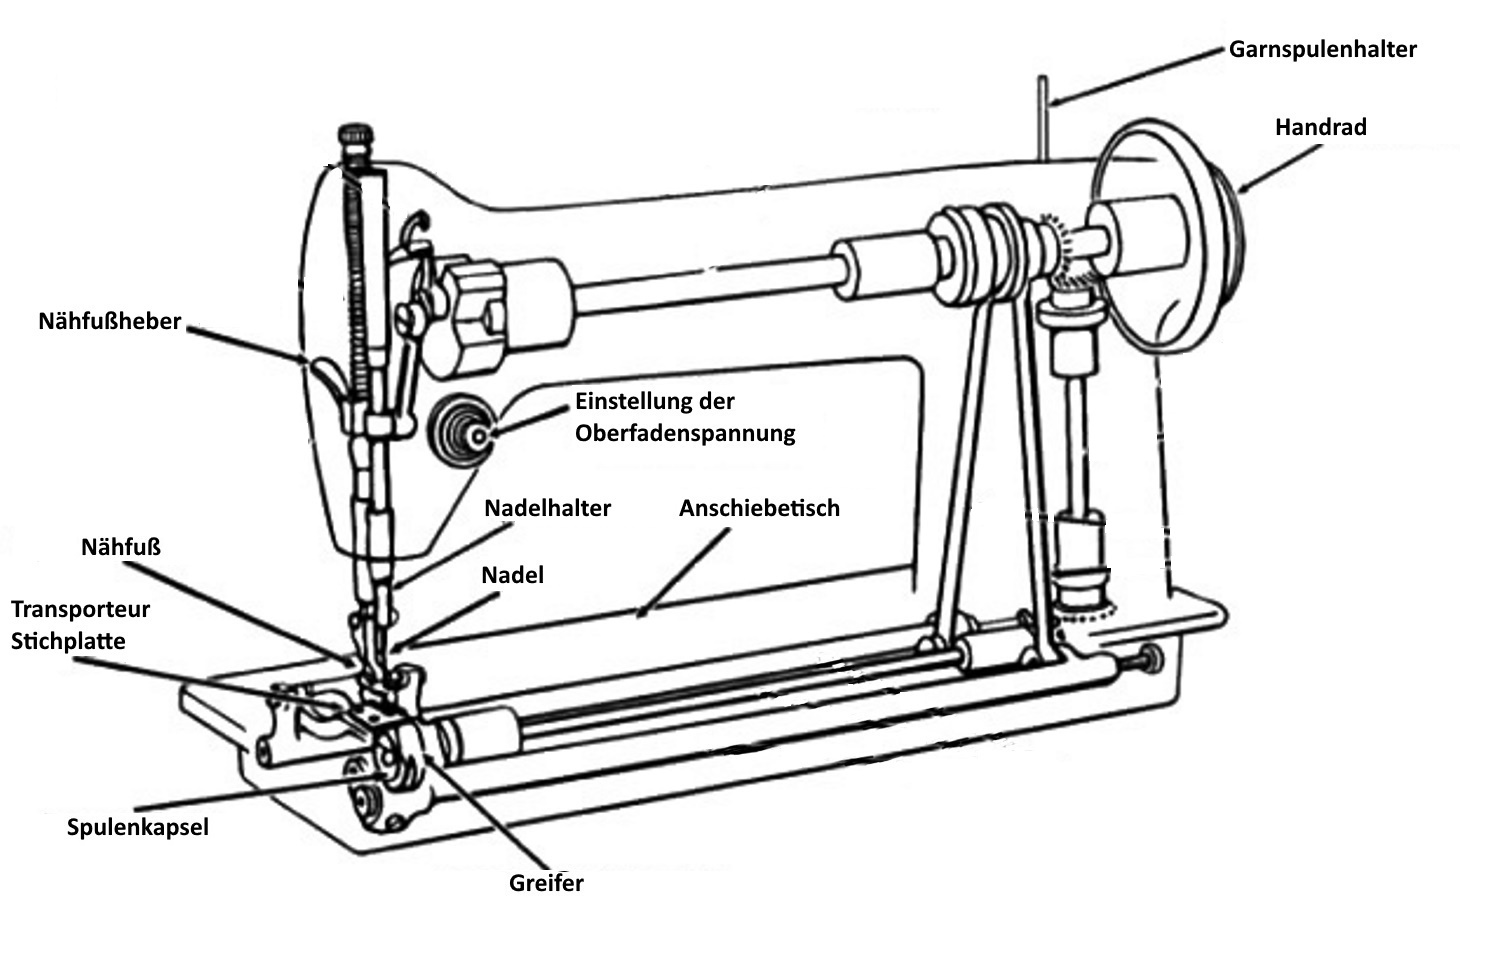
\includegraphics[width=\linewidth]{naehmaschine_wichtige_teile.jpg}

\subsection{Regeln und Hinweise}
\begin{itemize}
	\item Achtet immer darauf, wo sich eure Finger befinden. Die Maschine näht viel schneller, als ihr im Notfall reagieren könnt. Nehmt beim hantieren im Nähbereich immer den Fuß vom Anlasser. Achtet beim Nähen darauf, immer genug Abstand zwischen der Nadel und euren Händen zu halten.
	\item Für jede Näharbeit die richtige und einwandfreie, nicht verbogene Nadel verwenden. Bei der Verwendung einer verbogenen Nadel, kann diese auf die Stichplatte treffen und dadurch der Mechanik der Maschine stark beschädigt werden.
	\item Den Stoff niemals schieben oder ziehen. Den Transport der Stoffes erledigt der sog. Transporteur für dich. Du musst musst lediglich den Stoff um die Nadel herum drehen, um die Richtung vorzugeben. Solltest du dennoch am Stoff ziehen oder ihn schieben, kann sich die Nadel mit den oben genannten Folgen verbiegen
	\item Nicht bei beschädigter Stichplatte nähen, sonst droht sonst kann sich die Nadel verbiegen/brechen (s.o.).
	\item Bevor ihr losnäht immer darauf, dass der Nähfuß abgesenkt ist. Der Nähfuß lässt sich mit dem Nähfußheber an der Rückseite der Maschine hbeen und senken. Solltet ihr bei angehobenem Nähfuß losnähen, werder ihr Fadensalat produzieren, der u.U. nur sehr aufwändig wieder entfernt werden kann.
	\item Nichts mit Gewalt verschieben, einsetzen, bewegen, verstellen! Die Mechanik ist leichtgängig bei korrekter Handhabung und Behandlung.
	
	\item Verschiedene Materialien erfordern die Verwendung verschiedener Nadelstärken (üblicherweise zwischen 60 und 110) und Nadeltypen (z.B. Stretch-, Jeans-,  Universalnadel, etc.)
	\item Schaltet die Maschine bei Arbeiten im Nadelbereich (Nadel wechseln, Nähfuß wechseln, etc.) aus.
	\item Ohne Rücksprache mit einem Betreuer darf niemals die Unterfadenspannung verändert werden.
	\item Achtet beim Nähen immer darauf, wie sich die Maschine verhält. Geräusche, Gerüche, Nadelbewegung oder Vibrationen, die euch bisher unbekannt waren, können auf Beschädigungen an der Maschine oder eine Fehlbedienung hinweisen. Bitte informiert, wenn euch etwas komisch vorkommt, immer eine*n Betreuer*in.
	\item Das Nählicht der Maschine wird mit Netzspannung (230V) betrieben. Die Glühbirne darf daher niemals bei in die Steckdose eingesteckter Maschine gewechselt werden. Andern falls droht Lebensgefahr durch einen elektrischen Schlag. Außerdem wird es während des Nähens sehr heiß. Achtet daher darauf, euch nicht daran zu verbrennen.
\end{itemize}


\subsection{Fragen/Vorführung Einweisung}
Folgende Dinge musst du für eine erfolgreiche Einweisung vorführen bzw. beantworten können:
\begin{itemize}
	\item Dinge, die du vorführen können solltest:
	\begin{itemize}
		\item Aufbauen, Überprüfen, Einschalten und Abbauen der Maschine
		\item Ölen des Umlaufgreifers
		\item Einsetzen der Nadel
		\item Spulen des Fadens auf die Unterfadenspule
		\item Einsetzen der Unterfadenspule in die Spulenkapsel, Überprüfung der Unterfadenspannung (falls diese nicht passt, Betreuer*in informieren)
		\item Einfädeln des Oberfadens
		\item Wechseln des Nähfußes
		\item Heraufholen des Unterfadens
		\item Anpassen der Obefadenspannung
		\item Umschalten zwischen Zickzack und Geradstich
		\item Einstellen der Stichlänge, Stichbreite
		\item Zustand, in dem du deinen Arbeitsplatz hinterlassen wirst
	\end{itemize}
	
	\item Fragen, die du beantworten können solltest:
\end{itemize}



\vspace{5em}
\hrule

Alles bis hier musst du auswendig wissen. Den Rest kannst du bei Bedarf nachschauen.
\vspace{0.2em}
\hrule
\vspace{3em}

\pagebreak
\section{Allgemeines}

\subsection{Vor dem Nähen/ Sticken}
\begin{itemize}
 \item Nähmaschine auf einen stabilen Tisch stellen, sodass sie \textbf{nicht wackelt} zusammen mit
 \begin{itemize}
 	\item[\pfeil] \textbf{beim Nähen:} angeschobener Zubehörbox
 	\item[\pfeil] \textbf{beim Sticken:} angeschobener Stickvorrichtung
 \end{itemize}
 \item Netzkabel anschließen (alles rechts an Maschine) und außerdem
  \begin{itemize}
 	\item[\pfeil] \textbf{beim Nähen:} Fußanlasser anschließen
 	\item[\pfeil] \textbf{beim Sticken:} PC und Stickmaschine via USB-Kabel verbinden
 \end{itemize}
\end{itemize}

\subsection{Nach dem Nähen/ Sticken}
\begin{itemize}
 \item Nähmaschine abschalten, bevor das Netzkabel getrennt wird
 \item Fußanlasser abziehen und getrennt aufräumen
 \item Nähfußheber in niedrigste Position bringen (Nähfuß ist komplett abgesenkt)
 \item nach dem Sticken: Stickaufsatz entfernen und Zubehörbox anschieben
\end{itemize}

\subsection{Teile der Maschine und Zubehör}

Eine Abbildung mit der Benennung aller Teile der Maschine findest du in der Gebrauchsanleitung auf S. 7-9. Lese dir diese durch und verinnerliche die Namen der Maschinenteile, um diese Einweisung zu verstehen.

\vspace{2em}

Folgende Fragen solltest du ohne Zögern beantworten können:
\begin{itemize}
 \item Welche Nähfüße gibt es? Welcher ist der Standard-Nähfuß?
 \item wo liegt der Transporteur und der Transportschalter?
 \item wo finde ich Näßfußheber und Einfädlerhebel?
 \item Wo wird die Unterfadenspule eingesetzt?
 \item Welche Klasse müssen die Unterfadenspulen haben?
\end{itemize}


\subsection{Nähfußheber}
Der Nähfußheber kann in drei Positionen gebracht werden:
\begin{itemize}
 \item \textbf{abgesenkt:} Position zum Nähen und Sticken
 \item \textbf{angehoben:} Position zum Einlegen und Entnehmen von Stoff 
 \item \textbf{manuell weiter angehoben (höchste Position):} wichtig zum Einlegen und Entfernen der Stickrahmen und bei voluminösen Stoff usw. \pfeil \textbf{nicht mit Gewalt den Nähfuß anheben oder Stickrahmen darunter schieben!}
\end{itemize}

\subsection{Transporteur anheben/ versenken}
Der Transporteur ist dafür zuständig, den Stoff beim Nähen automatisch weiterzuschieben, zu \textbf{transportieren}. 
\newline Beim Sticken und Annähen von Knöpfen muss dieser versenkt werden:
\begin{itemize}
 \item entfernen des Zubehörfaches durch Schieben nach links
 \item Hebel an der Rückseite auf jeweiliges Zeichen stellen (evtl erst leicht nach unten drücken, dann auf jeweilige Seite schieben):
	\begin{itemize}
 	 \item \textbf{“Zähnchen unter Strich”:} Transporteur versenkt, Stoff wird nicht automatisch
transportiert, wichtig zum Annähen von Knöpfen und beim Sticken
 	 \item Wird das Stickaggregat angebracht, wird der Transporteur automatisch versenkt. Er muss anschließend wieder angehoben werden! (Siehe “Sticken”)
 	 \item \textbf{“Zähnchen über Strich”:} Transporteur angehoben, Stoff wird automatisch transportiert 
	\end{itemize}
\end{itemize}

\subsection{Nadeln}
\textcolor{red}{Wichtig:} Unbedingt einwandfreie Nadeln verwenden: gute Qualität, gerade, nicht abgebrochen, schlägt nicht an, usw.!
\begin{itemize}
 \item \textbf{Normales Nähen:} Universalnadeln
 \item \textbf{Sticken:} Sticknadeln (“schärfer”), roter Strich
 \item \textbf{evtl:} Stretchnadeln (“runde Spitze” gelber Strich), Jeansnadeln (blauer Strich) usw.
\end{itemize}

\vspace{2em}

\textbf{Nadel wechseln:}
\newline \textbf{Anleitung S.21 oder zeigen lassen}
\begin{itemize}
 \item[\pfeil] Nähfuß anheben
 \item[\pfeil] Nadel in höchste Stellung mit Handrad bringen
 \item[\pfeil] Schraube rechts an Nadel mit Zubehörwerkzeug öffnen
 \item[\pfeil] Nadel entfernen (nicht einfach herausfallenlassen, sondern herausnehmen)
 \item[\pfeil] Nadel mit abgeflachter Seite nach hinten einlegen
 \item[\pfeil] Nadel bis zum Anschlag nach oben schieben
 \item[\pfeil] Schraube festdrehen -  fest, aber ohne Gewalt
\end{itemize}

\subsection{Nähfuß wechseln}
\textcolor{red}{Es gibt verschiedene Nähfüße, je nach Zweck müssen diese gewechselt werden! }
\newline z.B. große Zierstiche, Reißverschluss, Knopfloch usw. 

\vspace{2em}

\textbf{Normalerweise:}
\begin{itemize}
 \item[\pfeil] Nähfuß angehoben, Nadel in höchster Position evtl. manuell
 \item[\pfeil] kleinen Hebel direkt hinten am Nähfuß drücken
 \item[\pfeil] Nähfuß abnehmen
 \item[\pfeil] neuen Nähfuß mittig auf Stichplatte zentrieren 
 \item[\pfeil] Nähfuß-Halterung senken und Nähfuß einrasten lassen
\end{itemize}

\vspace{2em}

\textbf{Anbringen/ Entfernen des Stickfußes:}
\newline
\textbf{Anleitung S. 65 oder zeigen lassen}
\begin{itemize}
 \item[\pfeil] Nadel in höchste Position evtl manuell, Nähfuß angehoben
 \item[\pfeil] Schraube links an Nähfuß-Halterung mit Zubehörwerkzeug öffnen
 \item[\pfeil] universal Nähfuß-Halterung entfernen und zu Zubehör legen
 \item[\pfeil] Stickfuß so anbringen, dass Hebel oberhalb Nadelbefestigung liegt
 \item[\pfeil] festschrauben, ohne Gewalt
 \item[\pfeil] Stickfuß liegt in abgesenkter Position nicht auf der Stichplatte auf!
\end{itemize}

\subsection{Oberfaden einfädeln}

\textcolor{red}{Nur bei angehobenem Fuß!}

\vspace{1em}

\textbf{Anleitung S.16 oder zeigen lassen}
\begin{itemize}
 \item senkrechten Stift aus Zubehör oben rechts einstecken, da eigentlicher Stift schlecht hält
 \item Garnrollen meist auf den senkrechten Stift aufstecken, evtl.Garnrollenführungsscheibe leicht aufstecken (Anleitung S.10)
 \item Nadeleinfädler verwenden siehe Anleitung S.18 \pfeil keine Gewalt, verstellt sich sehr leicht! (zur Not per Hand einfädeln, Garn muss von vorne nach hinten laufen)
\end{itemize}

\vspace{2em}

\textbf{Test auf richtiges Einfädeln:}
\begin{itemize}
 \item[\pfeil] Einfädeln
 \item[\pfeil] Nähfuß angehoben lassen
 \item[\pfeil] den Faden leicht nach hinten weg ziehen \pfeil wenig Widerstand!
 \item[\pfeil] Nähfuß absenken
 \item[\pfeil] den Faden leicht nach hinten weg ziehen \pfeil Widerstand, Nadel biegt sich leicht (nicht gegen Widerstand ziehen!)
\end{itemize}

\subsection{Unterfaden einfädeln}
\textcolor{red}{Immer normales Nähgarn als Unterfaden, nie Stickgarn verwenden!}

\vspace{1em}
\textbf{Anleitung S.14 oder zeigen lassen}
\begin{itemize}
 \item[\pfeil] Nadel in die höchste Position bringen
 \item[\pfeil] Spulenabdeckung entfernen
 \item[\pfeil] Spule so einlegen, dass sich der Faden gegen den Unterzeigersinn abrollt
 \item[\pfeil] Faden in den Schlitz und in die Führung legen bis zur Stichplatte und am Fadenabschneider abschneiden
\end{itemize}

\subsection{Spulen}
\textbf{Anleitung S.12 oder zeigen lassen}
\begin{itemize}
 \item[\pfeil] passende Spulen verwenden
 \item[\pfeil] Spule auf den Spuler drücken
 \item[\pfeil] Faden nach Anleitung einfädeln und einige Male per Hand um die Spule wickeln oder durch das Loch in der Spule fädeln
 \item[\pfeil] Spulenhebel gegen die Spule drücken \pfeil Spule dreht sich bis sie voll ist oder manuell Hebel wegdrücken
 \item[\pfeil] Faden abschneiden, Spule abnehmen
\end{itemize}

\pagebreak
\section{Nähen}

\textcolor{red}{Prinzipiell näht und die stickt die Maschine mit der eingestellten Fadenspannung sehr gut! }
\textcolor{red}{\newline \pfeil Ohne Rücksprache mit einem Betreuer niemals die Fadenspannung ändern!}

\vspace{1em}

\textcolor{red}{Die Maschine zeigt auf dem Display auch alle aufgetretenen Fehler an, falls dies der Fall ist: \textbf{Fragen!}}


\subsection{Stichart einstellen}
\textbf{Anleitung S. 27, alle möglichen Stiche sind auf dem Musterbogen abgedruckt}
\begin{itemize}
 \item Stiche werden im Display angezeigt (der Punkt zeigt Nadelposition der Grundeinstellung des ausgewählten Stiches an)
 \item oberes Wahlrad drehen wechselt die Stiche, oberes Rad drücken springt in 10er Schritten durch die Stiche
 \item unteres Wahlrad: obere LED leuchtet: Stichbreite bzw. Nadelposition wird geändert
 \item Durch Drücken des unteren Wahlrades: untere LED leuchtet: Stichlänge wird geändert
\end{itemize}

\subsection{Sonstige Nähfunktionen}
\textbf{Anleitung S. 33}
\begin{itemize}
 \item \textbf{Vernähen:} Faden wird vernäht und löst sich nicht mehr, wichtig am Anfang und Ende des Nähens, bei Geradstichen auch mit Rückwärtstaste
 \item \textbf{Fadenabschneider:} schneidet automatisch Ober- und Unterfaden ab
 \item \textbf{Nadel ``hoch'' / ``tief'':} LED oben leuchtet \pfeil bei Loslassen des Anlassers ist Nadel oben, LED unten leuchtet \pfeil bei Loslassen des Anlassers bleibt Nadel unten im Stoff stecken 
 \item \textbf{Rückwärtstaste:} näht automatisch 5 Stiche rückwärts, zB bei Geradstich, Zickzack
 \item \textbf{Start/Stop Taste:} nur wichtig beim Sticken (Startet Stickvorgang)
 \item \textbf{Speed:} hauptsächlich wichtig beim Sticken (Geschwindigkeit), steuert aber Empfindlichkeit des Fußanlassers! \textcolor{red}{Höchstens mittlere Geschwindigkeit einstellen!}
\end{itemize}

% schoenere Darstellung
\newpage
\ccLicense{naehmaschine-einweisung}{Einweisung Nähmaschine}

\end{document}
